In this chapter a search for highly ionizing, short tracks is presented. The chapter will be structured as follows:
In \mbox{Sec.~\ref{sec:Motivation}} a motivation will be given, followed by an overview of the general search strategy in \mbox{Sec.~\ref{sec:GeneralSearchStrategy}}.
As the variable \dedx plays a crucial role in this analysis, a general introduction and different possible parametrizations will be introduced in \mbox{Sec.~\ref{sec:DeDxMeasurement}}.
In this context also the conducted offline calibration of the silicon pixel detector will be explained.
After presenting the simulated SM and signal samples which were used in this analysis (\mbox{Sec.~\ref{sec:SimulatedSamples}}) the event selection is shown (Sec.~\ref{sec:EventSelection}).
Then, the various sources of background are charecterized (Sec.~\ref{sec:SourcesOfBackgrounds}) and the methods to estimate their size are presented (\ref{sec:BackgroundEstimation}).
As a final step an optimization in the search sensitivity was done, which can be found in Sec.~\ref{sec:Optimization}.
The chapter concludes by presenting the results of this analysis in Sec.~\ref{sec:Results}, and after a short introduction to the statistical methods of limit setting (Sec.~\ref{sec:LimitSetting}), the results will be interpreted in the context of Supersymmetry (Sec.~\ref{sec:Interpretation}).


%%%%%%%%%%%%%%%%%%%%%%%%%%%%%%%%%%%%%%%%%%%%%%%%%%%%%%%%%%%%%%%%%%%%%%%%%%%%%%%%%%%%%%%%%%%%%%%%%%%%%%%%%%%%%%%%%%%%%%%%%%%%%%%%%%%%%%%%%%%%%%%%%%%%%%%%%%%%%%%%%%%%%%%%%%%%%%%%%%%%
\section{Motivation}
\label{sec:Motivation}
As it was already pointed out in Chap.~\ref{ch:Theory}, Supersymmetry is able to offer solutions to unexplained phenomena in astrophysics and can solve the shortcomings of the Standard Model of particle physics.
Unfortunately, due to the unknown mechanism of supersymmetry breaking, the most general parametrization of Supersymmetry introduces over 120 new dimensions which opens up an incredibly huge phenomenalogically rich space, 
leading to very different possible signature at particle colliders. 
During the Phase\,I run at the LHC in 2012, a variety of different seaches, optimized on the hunt for supersymmetry were conducted.
At the CMS experiment, taking data from proton-ptoton collsions, a strong focus was put on the search for hints of SUSY in the strong production sector (e.g. \cite{}).
This led already to a wide exclusion of SUSY space. 
Therefore, there is the need to focus on more ``exotic'' sectors, which cannot be easily accessed and require to design searches for very specialized signatures.
Among those signatures are SUSY models containing long-lived charginos. 
There have been already several analyses conducted in CMS which are in principle (even not all were designed to be) sensitive to these models.
The excluded space is shown in Fig.~\ref{fig:pMSSMplot}. 
\begin{itemize}
\item Explain pMMSM (give refenrence)
\item Explain what is shown in the plot
\item Explain more!
\end{itemize}

\begin{figure}[!ht]
  \centering 
  \begin{tabular}{c}
    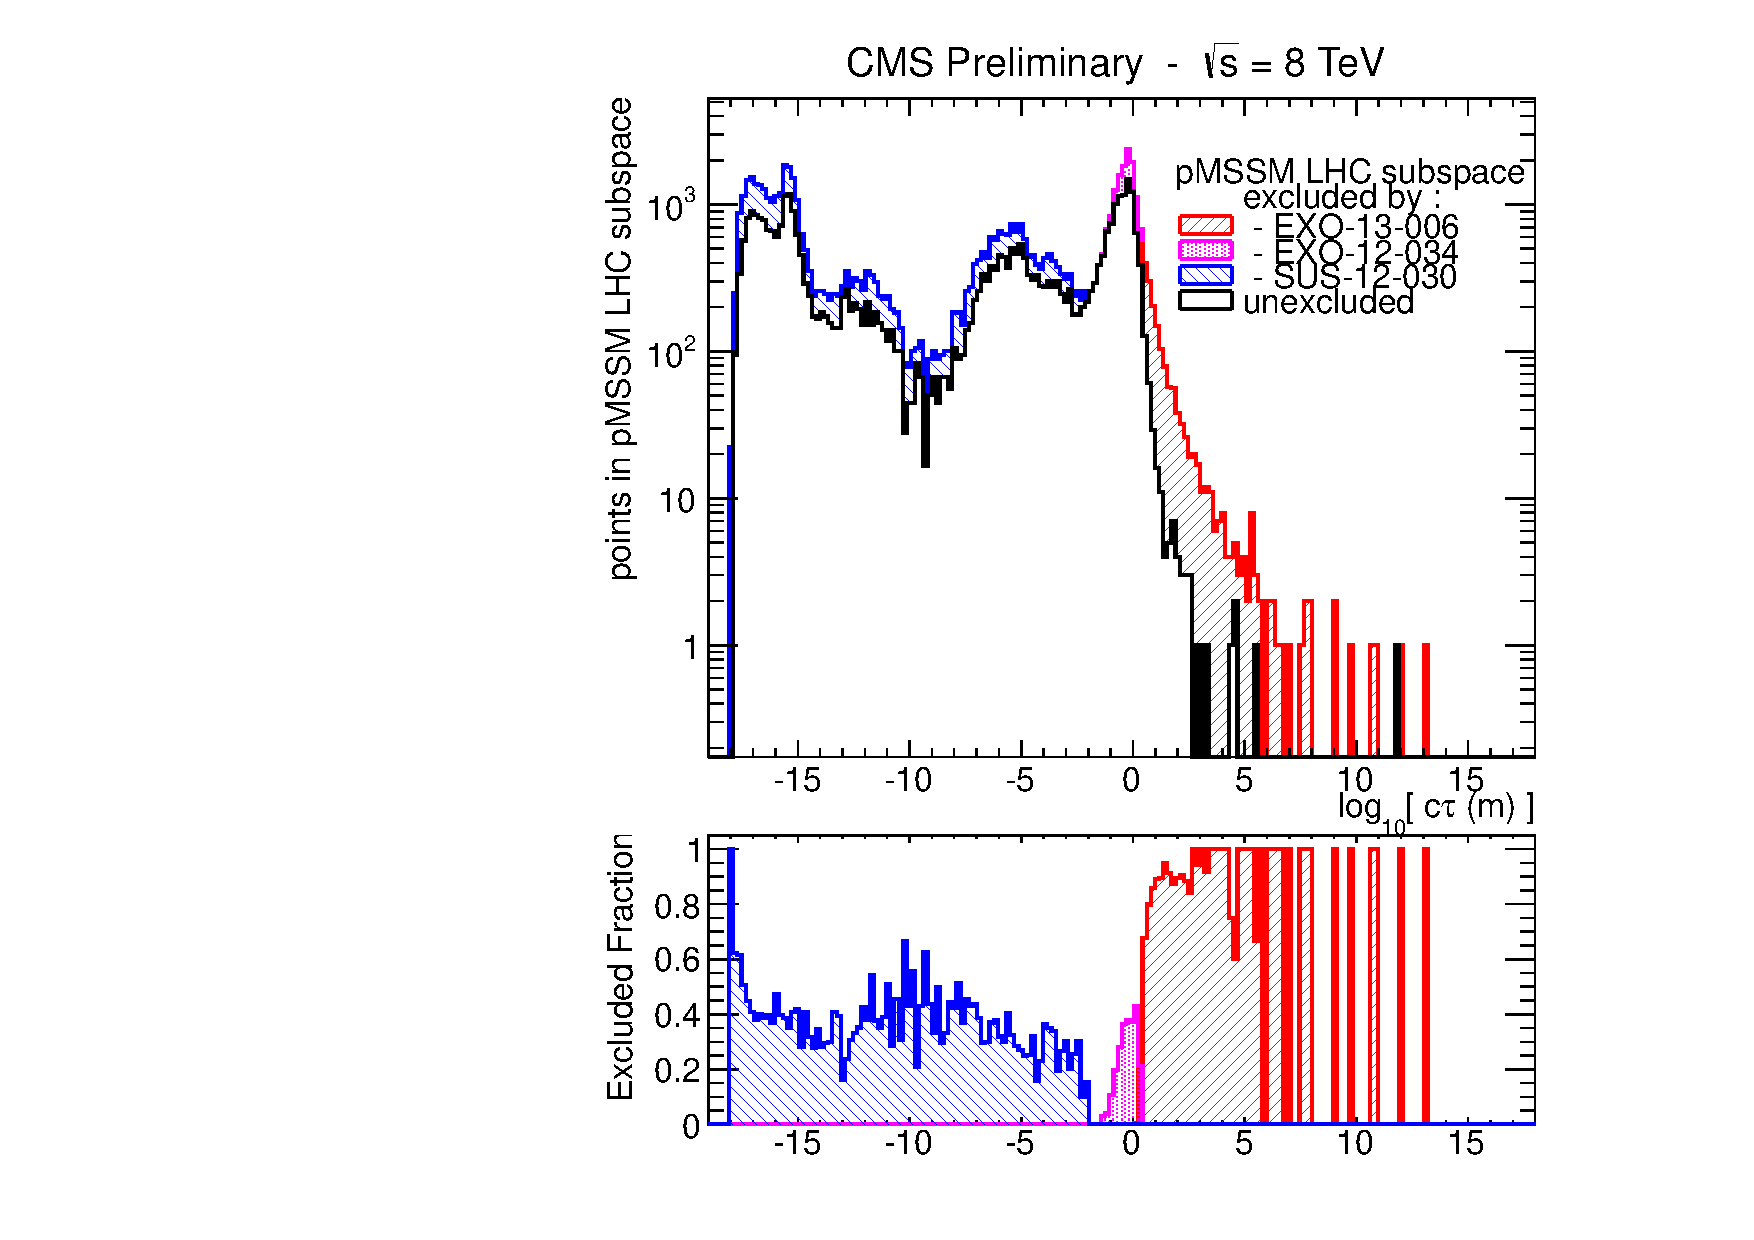
\includegraphics[width=0.75\textwidth]{figures/analysis/pMSSM_vs_ctau.pdf}
  \end{tabular}
  \caption{Exclusion power of various analyses dependent on chargino lifetime [c$\tau$]. Lower part of the plot shows the excluded fraction. Taken from: https://twiki.cern.ch/twiki/bin/view/CMSPublic/PhysicsResultsEXO12034}
  \label{fig:pMSSMplot}
\end{figure}

The analysis presented in this chapter is motivated by the possible existence of long-lived charginos, not decaying instantaneously but reaching the detector before their decay.
As shown in Sec.~\ref{bla bla}, long lifetimes are possible for various reasons. 
In this analysis the focus is put on the possiblity of a lightest chargino ($\chi^{\pm}_1$) which is almost mass degenerate with the lightest neutralino ($\chi^{0}_1$), leading in this case to long chargino lifetimes because of phase space supression.

A chargino can be produced via chargino pair production through a photon or a Z boson exchange. The chargino decays then via a virtual W boson to the lightest neutralino and fermion.
This process is illustrated in the Feynman diagram showed in fig. \ref{fig:FeynmanDiagram}.
\begin{figure}[!ht]
  \centering 
  \begin{tabular}{c}
    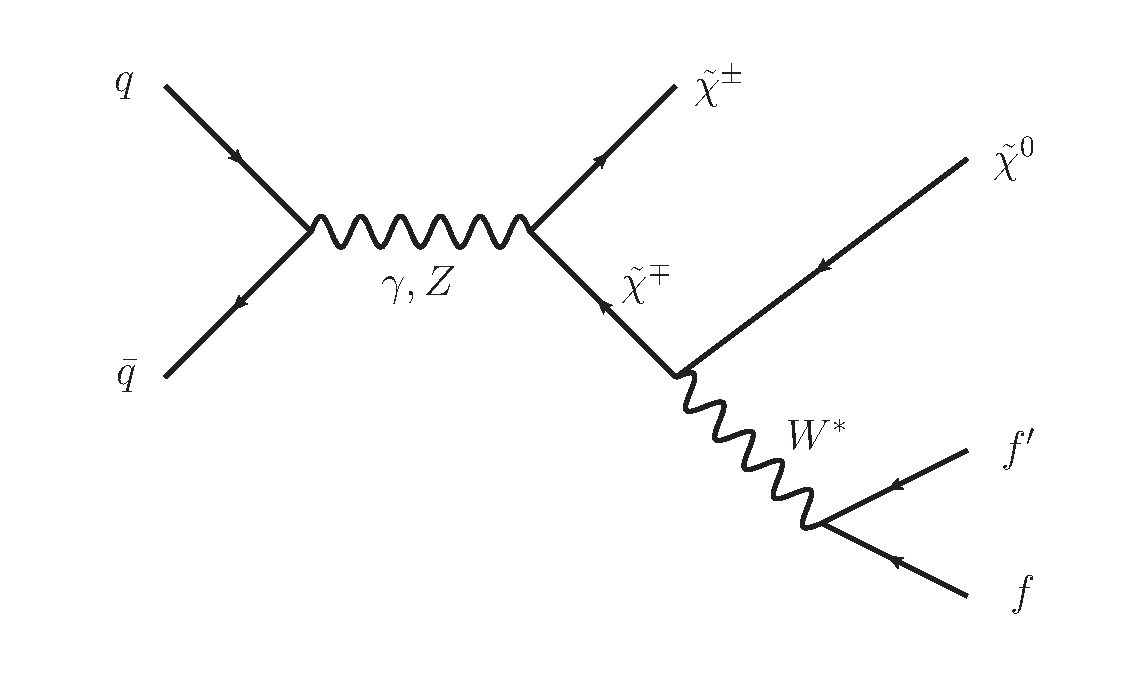
\includegraphics[width=0.75\textwidth]{figures/analysis/ChiChi_ProductionAndDecay.pdf}
  \end{tabular}
  \caption{Feynman diagram showing a possible production mechanism and the decay channel of a chargino.}
  \label{fig:FeynmanDiagram}
\end{figure}
Other possible production channels are the exchange of a supersymmetric Higgs boson or via a t-channel squark exchange. 
The corresponding Feynman diagrams for main production channels are shown in Fig.~\ref{fig:FeynmanDiagramProductionCharginoPair}.
\begin{figure}[!hb]
  \centering 
  \begin{tabular}{c}
    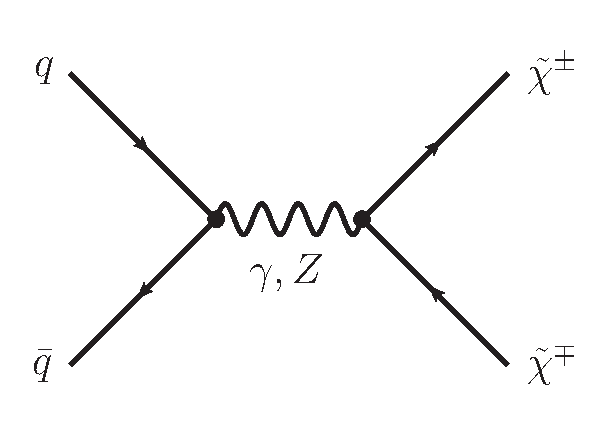
\includegraphics[width=0.33\textwidth]{figures/analysis/ChiChi_GammaZ.pdf}
    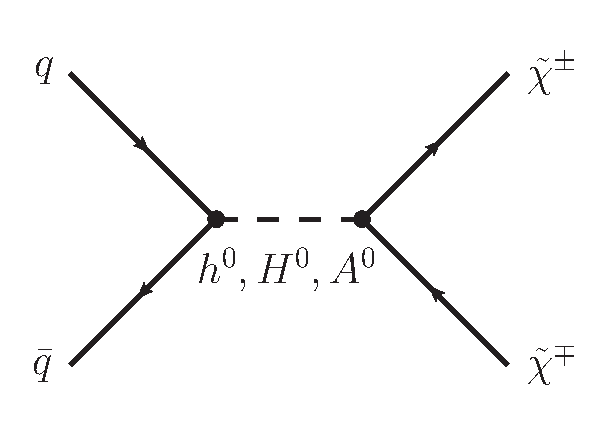
\includegraphics[width=0.33\textwidth]{figures/analysis/ChiChi_Scalar.pdf}
    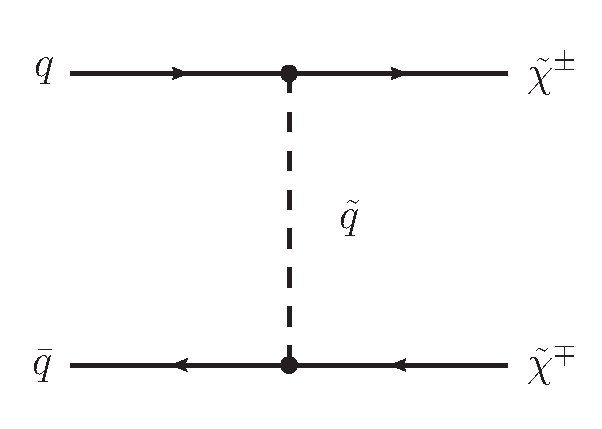
\includegraphics[width=0.33\textwidth]{figures/analysis/ChiChi_Squark.pdf}
  \end{tabular}
  \caption{Main tree level diagrams for chargino pair production.}
  \label{fig:FeynmanDiagramProductionCharginoPair}
\end{figure}
Another possibility of chargino production is the chargino neutralino production channel. 
On tree level, there exists the s-channel W boson exchange or the t-channel squark exchange, see Fig.~\ref{fig:FeynmanDiagramProductionCharginoNeutralino} for the Feynman diagrams.
\begin{figure}[!hb]
  \centering 
  \begin{tabular}{c}
    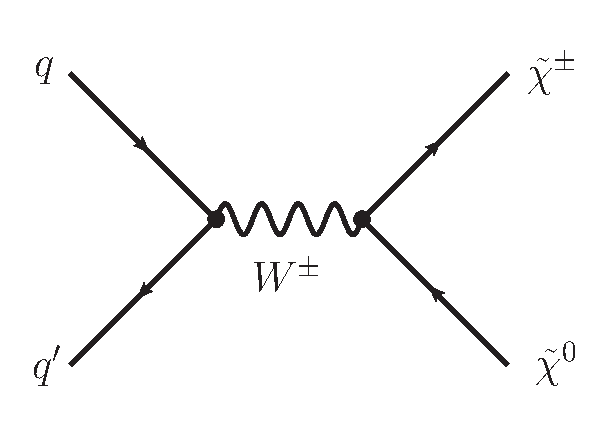
\includegraphics[width=0.33\textwidth]{figures/analysis/ChiChi0_WBoson.pdf}
    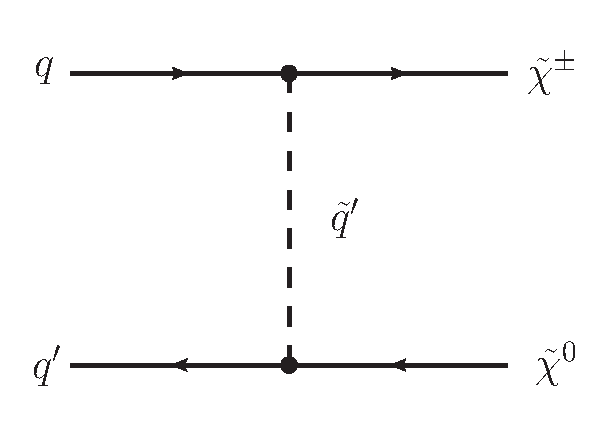
\includegraphics[width=0.33\textwidth]{figures/analysis/ChiChi0_Squark.pdf}
  \end{tabular}
  \caption{Main tree level diagrams for chargino neutralino production.}
  \label{fig:FeynmanDiagramProductionCharginoNeutralino}
\end{figure}









\begin{comment}
The search presented here aims to look for charged particles which decay inside the detetcor to a low momentum fermion and another only weakly interacting particle which is not visible inside the detector.
In the context of supersymmetry this charged particle can be the lightest chargino ($\tilde{\chi}^{\pm}_{1}$) which is almost mass-degenrate with the lightest neutralino ($\tilde{\chi}^{0}_{1}$), 
thus leading to another low-momentum fermion, which can be hardly reconstructed as a track because of its low \pt.



In case the chargino and the lightest neutralino are almost mass-degenerate the fermion is very low in momentum and can therefore be hardly detected in the tracker. 
The momentum of the fermion is of course highly dependent on the actual mass gap between the neutralino and the chargino. 
The typical \pt distribution of a pion when the mass gap is about the pion mass is shown in figure \ref{bla bla}








Being in principle sensitive to any physics beyond the standard model, this search is motivated by the possible existence of a supersymmetric chargino.



There are many analyses done at CMS which are in principle sensitive to such a supersymmetric chargino. 
This analyis wants to focus on long lifetimes such that the chargino does not directly decay, but reaches at least to first layers of the detector, being the silicon pixel and strip trackers. 
On the other hand, it has been designed in a way, that the chargino is not that-lonmg lived, that it travels through the whole detector, but decays at least before the muon chambers, thus is not reconstructed as a muon.
%There have been analysis at CMS and Atlas looking for such middel-live charginos. 
%The new aspect of the analysis is the inclusion of the variable dE/dx.
%The pixel and the silicon tracker at CMS have been calibrated already offline, when building these moduls. Unfortunately it is not so good.
%The silicon strip tracker has been calibrated in the context of a search for heavy, stable charged particle (cite something).
%In this analysis, also very short tracks become very important, showing not more than three of four hits. Therfore also the pixel detector needs to bec calibrated in order to increase senssitivy for those short tracks
\end{comment}

%%%%%%%%%%%%%%%%%%%%%%%%%%%%%%%%%%%%%%%%%%%%%%%%%%%%%%%%%%%%%%%%%%%%%%%%%%%%%%%%%%%%%%%%%%%%%%%%%%%%%%%%%%%%%%%%%%%%%%%%%%%%%%%%%%%%%%%%%%%%%%%%%%%%%%%%%%%%%%%%%%%%%%%%%%%%%%%%%%%%
\section{General search strategy}
\label{sec:GeneralSearchStrategy}
\begin{itemize}
\item No detection of low momentum fermions possible (fermion pt plot?)
\item Show event displays and sketch for pion decyay!
\item Detection via ISR 
\item Event selection by ISR jet and MET
\item Detection of track (possibly short and disappearing and highly ionizing, not reconstructed as muon)
\item Short and highly ionizing track $\rightarrow$ inclusion of pixel tracker information 
\end{itemize}

\begin{figure}[!tp]
  \centering 
  \begin{tabular}{c}
    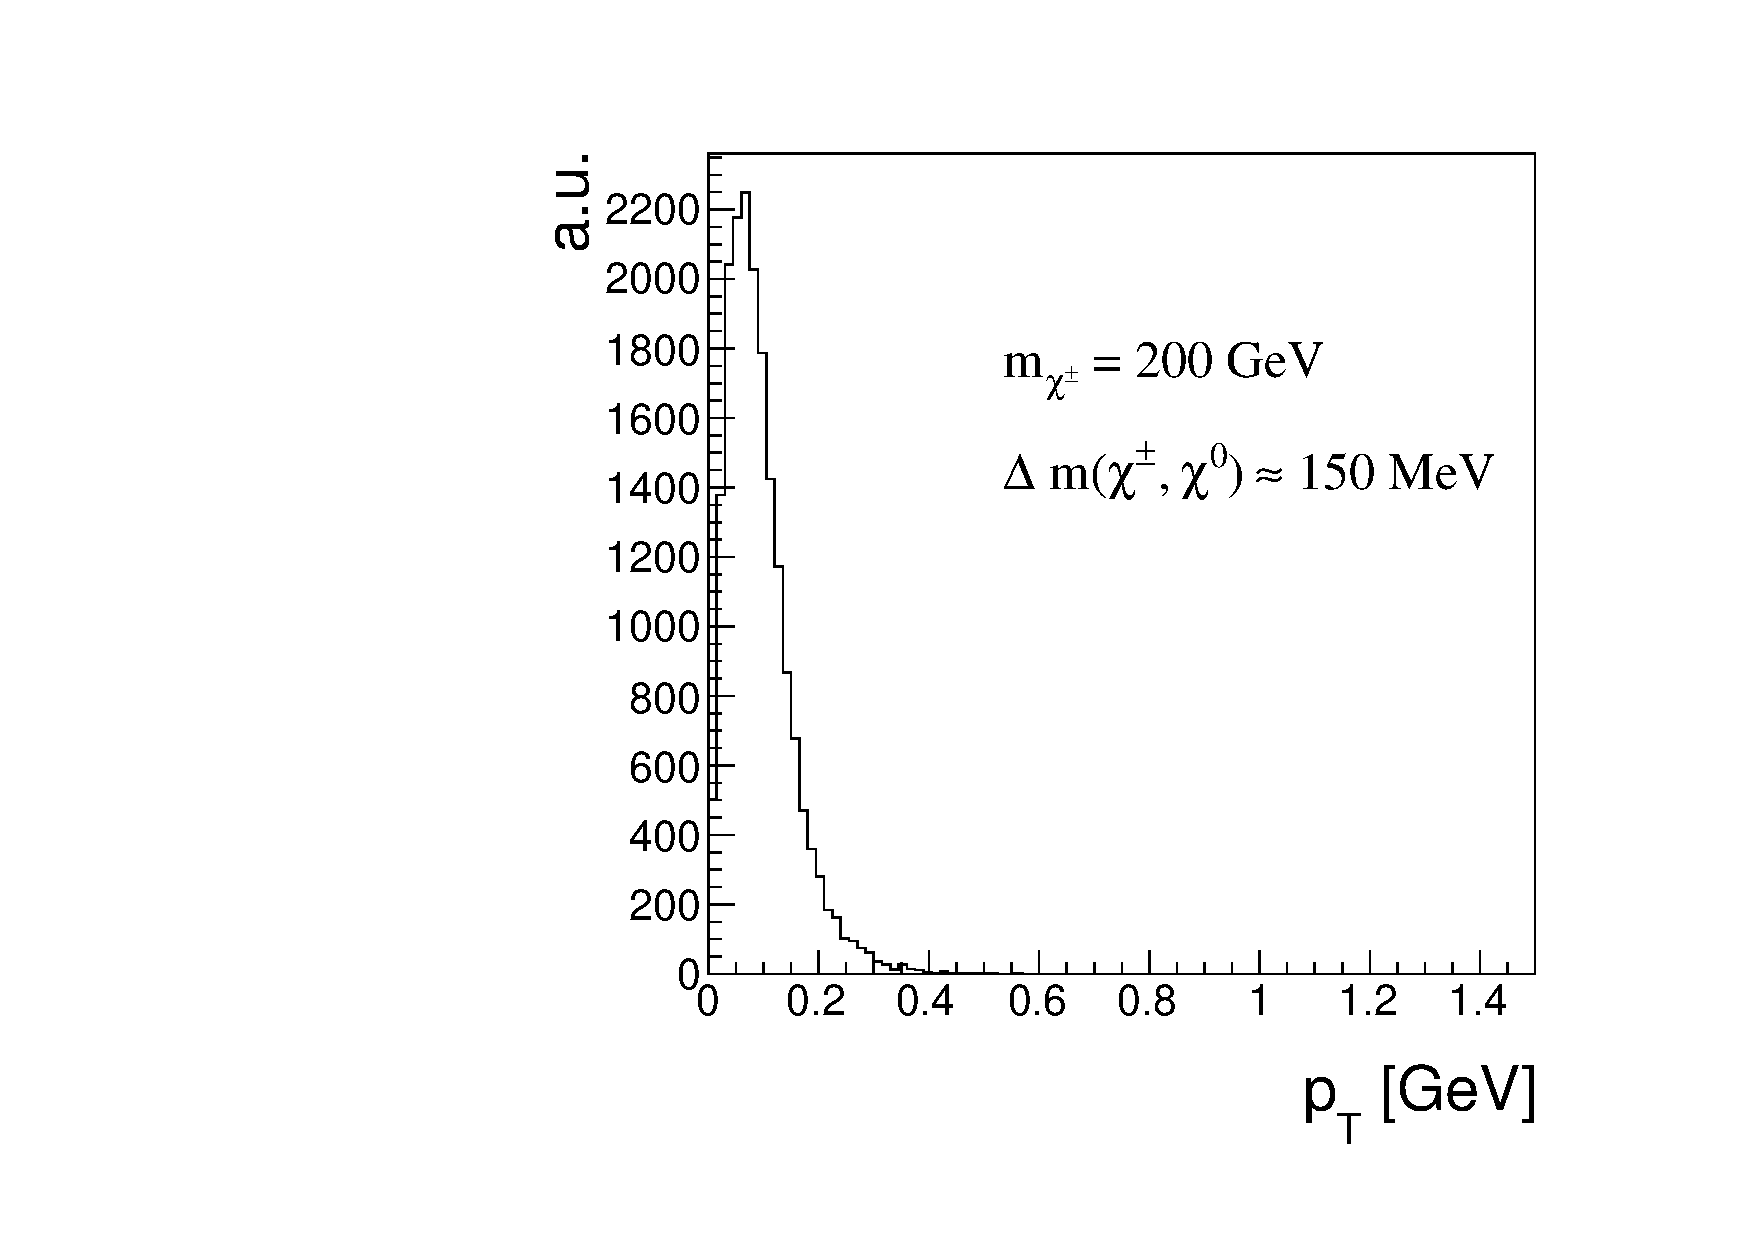
\includegraphics[width=0.85\textwidth]{figures/analysis/ptOfPions.pdf}
  \end{tabular}
  \caption{Transverse momentum distribution of pions coming from chargino decay into a neutralino with a mass gap of 150\mev.}
  \label{fig:ptOfPions}
\end{figure}


\subsection{Comparison to existing searches}
\begin{itemize}
\item HSCP
\item Disappearing track
\item No cut on Nhits
\item Muon veto + inclusion of dE/dx
\end{itemize}

%%%%%%%%%%%%%%%%%%%%%%%%%%%%%%%%%%%%%%%%%%%%%%%%%%%%%%%%%%%%%%%%%%%%%%%%%%%%%%%%%%%%%%%%%%%%%%%%%%%%%%%%%%%%%%%%%%%%%%%%%%%%%%%%%%%%%%%%%%%%%%%%%%%%%%%%%%%%%%%%%%%%%%%%%%%%%%%%%%%%
\section{(Improved) dE/dx measurement of short tracks}
\label{sec:DeDxMeasurement}
\subsection{Measuring dE/dx}
\begin{itemize}
\item The variable dE/dx: General introdution, Bethe-Bloch, 
\item Asymmetric Smirnov Discriminator
\end{itemize}
\subsection{Gain calibration of the silicon pixel tracker}
\subsection{Asymmetric Smirnov discriminator}
\subsection{Efficiency improvements}

%%%%%%%%%%%%%%%%%%%%%%%%%%%%%%%%%%%%%%%%%%%%%%%%%%%%%%%%%%%%%%%%%%%%%%%%%%%%%%%%%%%%%%%%%%%%%%%%%%%%%%%%%%%%%%%%%%%%%%%%%%%%%%%%%%%%%%%%%%%%%%%%%%%%%%%%%%%%%%%%%%%%%%%%%%%%%%%%%%%%
\section{Simulated samples}
\label{sec:SimulatedSamples}
\subsection{SM samples}
\subsection{Signal samples}

%%%%%%%%%%%%%%%%%%%%%%%%%%%%%%%%%%%%%%%%%%%%%%%%%%%%%%%%%%%%%%%%%%%%%%%%%%%%%%%%%%%%%%%%%%%%%%%%%%%%%%%%%%%%%%%%%%%%%%%%%%%%%%%%%%%%%%%%%%%%%%%%%%%%%%%%%%%%%%%%%%%%%%%%%%%%%%%%%%%%
\section{Event selection}
\label{sec:EventSelection}
\subsection{Datasets and triggers}
\begin{itemize}
\item Datasets and triggers used in the analysis
\item signal samples generated with Madgraph and pythia
\item They are decayed in Geant to only pions. Around ten different lifetimes were simulated
\item For other lifetimes: lifetime reweighting is done PLOT
\item For five diffenrent masses (100-500 GeV) 
\end{itemize}
\subsection{Preselection}
\begin{itemize}
\item Motivate different selection cuts
\item Reference DT search for most of them
\end{itemize}
\subsection{Main discriminating variables}
\begin{itemize}
\item dE/dx
\item pt
\item Show some MC signal bkg comparioson plots (only Wjets?)
\end{itemize}

%%%%%%%%%%%%%%%%%%%%%%%%%%%%%%%%%%%%%%%%%%%%%%%%%%%%%%%%%%%%%%%%%%%%%%%%%%%%%%%%%%%%%%%%%%%%%%%%%%%%%%%%%%%%%%%%%%%%%%%%%%%%%%%%%%%%%%%%%%%%%%%%%%%%%%%%%%%%%%%%%%%%%%%%%%%%%%%%%%%%
\section{Sources of backgrounds}
\label{sec:SourcesOfBackgrounds}
\begin{itemize}
\item Background consist of particles which make high energy deposits and are high pt
\item In general: Low background search
\end{itemize}
\subsection{Fake tracks}
\begin{itemize}
\item Definition of fake tracks
\item How can they fake the signal
\end{itemize}
\subsection{Muons}
\begin{itemize}
\item How can muons fake the signal
\end{itemize}
\subsection{Pions}
\begin{itemize}
\item How can pions fake the signal
\end{itemize}
\subsection{Electrons}
\begin{itemize}
\item How can electrons fake the signal
\end{itemize}

%%%%%%%%%%%%%%%%%%%%%%%%%%%%%%%%%%%%%%%%%%%%%%%%%%%%%%%%%%%%%%%%%%%%%%%%%%%%%%%%%%%%%%%%%%%%%%%%%%%%%%%%%%%%%%%%%%%%%%%%%%%%%%%%%%%%%%%%%%%%%%%%%%%%%%%%%%%%%%%%%%%%%%%%%%%%%%%%%%%%
\section{Background estimation methods}
\label{sec:BackgroundEstimation}
\subsection{Fake background}
\subsection{Leptonic background}
\subsection{Systematic uncertainties}

%%%%%%%%%%%%%%%%%%%%%%%%%%%%%%%%%%%%%%%%%%%%%%%%%%%%%%%%%%%%%%%%%%%%%%%%%%%%%%%%%%%%%%%%%%%%%%%%%%%%%%%%%%%%%%%%%%%%%%%%%%%%%%%%%%%%%%%%%%%%%%%%%%%%%%%%%%%%%%%%%%%%%%%%%%%%%%%%%%%%
\section{Optimization of search sensitivity}
\label{sec:Optimization}
\begin{itemize}
\item Show plots
\item show table
\item Include NlostOuter here, too
\end{itemize}

%%%%%%%%%%%%%%%%%%%%%%%%%%%%%%%%%%%%%%%%%%%%%%%%%%%%%%%%%%%%%%%%%%%%%%%%%%%%%%%%%%%%%%%%%%%%%%%%%%%%%%%%%%%%%%%%%%%%%%%%%%%%%%%%%%%%%%%%%%%%%%%%%%%%%%%%%%%%%%%%%%%%%%%%%%%%%%%%%%%%
\section{Statistical Methods/ Limit setting}
\label{sec:LimitSetting}

%%%%%%%%%%%%%%%%%%%%%%%%%%%%%%%%%%%%%%%%%%%%%%%%%%%%%%%%%%%%%%%%%%%%%%%%%%%%%%%%%%%%%%%%%%%%%%%%%%%%%%%%%%%%%%%%%%%%%%%%%%%%%%%%%%%%%%%%%%%%%%%%%%%%%%%%%%%%%%%%%%%%%%%%%%%%%%%%%%%%
\section{Results}
\label{sec:Results}
\begin{itemize}
\item Data cutflowtable
\item Tables with results
\item One plot (4 bins: Prediction and data)
\end{itemize}

%%%%%%%%%%%%%%%%%%%%%%%%%%%%%%%%%%%%%%%%%%%%%%%%%%%%%%%%%%%%%%%%%%%%%%%%%%%%%%%%%%%%%%%%%%%%%%%%%%%%%%%%%%%%%%%%%%%%%%%%%%%%%%%%%%%%%%%%%%%%%%%%%%%%%%%%%%%%%%%%%%%%%%%%%%%%%%%%%%%%
\section{Interpretation}
\label{sec:Interpretation}
\subsection{Systematic uncertainties of simulated signal samples}
\subsection{Exclusion limits}
\begin{itemize}
\item 1-d limits
\item 2-d limits
\end{itemize}

